% DRAFT. The official NeurIPS 2026 style exists (neurips_2026.sty in the archive
% https://media.neurips.cc/Conferences/NeurIPS2026/Formatting_Instructions_For_NeurIPS_2026.zip,
% checked: HTTP 200, contains neurips_2026.tex, neurips_2026.sty, checklist.tex).
% The file has NOT been copied into the repository. If neurips_2026.sty is present alongside, it is loaded;
% otherwise a plain article skeleton is used (REPLACE WITH THE OFFICIAL STYLE before submission).
\documentclass{article}
\IfFileExists{neurips_2026.sty}{\usepackage{neurips_2026}}{%
  \usepackage[margin=1in]{geometry}\newcommand{\And}{\quad}\newcommand{\AND}{\\}}
\usepackage[utf8]{inputenc}
\usepackage[T1]{fontenc}
\usepackage{amsmath,amssymb,booktabs,hyperref,xcolor,enumitem}
\newcommand{\todo}[1]{\textcolor{red}{[TODO: #1]}}
\newcommand{\tbd}{\textcolor{red}{TBD}}
\newcommand{\E}{\mathbb{E}}
\newcommand{\Var}{\mathrm{Var}}

\title{Noise Ceilings for Molecular Property Benchmarks:\\ How Much of Model Ranking Lies Inside Measurement Noise?}
\author{Anonymous authors \\ \todo{authors; anonymity per track rules, not verified}}

\begin{document}
\maketitle
\begin{abstract}
The same compound measured against the same target in different laboratories often receives different potency values, which limits how well any model can be scored against such labels. For 17 potency tasks (target $\times$ $K_i$ or $\mathrm{IC}_{50}$) from ChEMBL~37, we estimate this limit per task from 3{,}292 molecules reported in at least two source documents and express model scores as a \emph{fraction of ceiling} $f$ (0: predicting the training mean; 1: reaching the estimated noise floor). The floors range from 0.31 to 0.79 pChEMBL units, but for some tasks the replicates come from a few document pairs, and a bootstrap over document pairs then gives intervals several times wider than one over molecules. After removing molecules found in MoleculeNet and TDC, we benchmark ECFP-based gradient boosting, random forest and MLP models and frozen ChemBERTa-77M and MoLFormer-XL embeddings with a boosted-tree head under random, scaffold and temporal splits. ECFP with a random forest reaches a mean $f$ of 0.90, 0.73 and 0.36 on the three splits (random: median 0.82, range 0.80--1.03 over the floor's uncertainty). The frozen embeddings reach 0.69/0.66, 0.55/0.54 and 0.25/0.25 (ChemBERTa/MoLFormer) and are below ECFP with gradient boosting on every split (Wilcoxon over tasks, Holm-adjusted $p<0.05$); on five tasks, a D-MPNN and a fine-tuned ChemBERTa do not close the gap on random and scaffold splits. On five task--split combinations ECFP models score below the estimated floor ($f>1$), which shows that the floor is uncertain for these tasks; we discuss mis-estimation and learnable document-level offsets as explanations. We report single-test-set minimum detectable effects and a reporting protocol, and release code and data.
\end{abstract}

\section{Introduction}
\paragraph{For chemists: what an ML benchmark and a split are.}
A machine-learning (ML) benchmark for molecular properties is a fixed table of molecules with measured values (the \emph{labels}), a rule for dividing it into a training part and a held-out test part (the \emph{split}), and a metric. Models learn from the training molecules and are scored on how well they predict the held-out ones; leaderboards then rank models by this score. The split determines what the score means: a \emph{random} split puts similar molecules on both sides and rewards interpolation; a \emph{scaffold} split keeps molecules sharing a core ring system on one side only, testing generalisation to new chemotypes; a \emph{temporal} split trains on older and tests on newer data, mimicking prospective use. A \emph{noise ceiling} is the best score any model could reach given that the labels themselves are imprecise.

\paragraph{For ML readers: the chemistry of the labels.}
Most public potency data originate in ChEMBL~\cite{zdrazil2023chembl}, a database manually curated from the literature. Potency is reported as $K_i$ (inhibition constant) or $\mathrm{IC}_{50}$ (concentration giving 50\% inhibition), both in molar units, and usually converted to the log-scale \emph{pChEMBL} value, $-\log_{10}$ of the molar value (a pChEMBL of 7 means 100\,nM). An \emph{assay} is one experimental protocol measuring a molecule against a target (enzyme, receptor or cell line) under specific conditions. A ChEMBL \emph{document} is one source publication (or deposited dataset) from which assays were extracted; different documents typically mean different laboratories, protocols and reagents. A learning \emph{task} here is a (target, measurement type) pair, e.g.\ human target X, $K_i$.

\paragraph{Problem.}
A molecule tested in two documents often receives different values~\cite{landrum2024combining}. If two models differ by less than this disagreement, a leaderboard gap says little about real predictive quality. Prior work estimates performance bounds by adding noise of an assumed size~\cite{crusius2025fitting}; we instead \emph{measure} the noise from actual replicate measurements across independent documents.

\paragraph{Contributions.}
(i) A replicate-based estimator of per-endpoint noise ceilings with molecule-level bootstrap and sensitivity analysis. (ii) A fraction-of-ceiling metric that makes scores comparable across endpoints. (iii) A dataset of replicated molecules decontaminated against existing benchmarks. (iv) A benchmark comparing tuned small models and frozen foundation-model embeddings under three splits and five seeds. (v) Recommendations: minimum detectable effect, a reporting protocol and a checklist. Whether any claimed advantage of pretrained embeddings survives is \tbd{}.

\paragraph{Hypotheses (to be tested, with refutation criteria).}
H1: between-document noise is comparable to model error on a substantial share of endpoints (refuted if ceilings are near perfect; then the noise argument does not hold and the paper is reframed as a model comparison). H2: the advantage of pretrained embeddings over ECFP+GBM shrinks or vanishes when measured as fraction of ceiling (refuted if it persists across splits with paired confidence intervals excluding zero). Both are untested.

\section{Related work}
Statements below are based on abstracts and search excerpts (see \texttt{docs/NOVELTY.md}); full texts must be read before submission \todo{read in full; re-run search incl.\ Polaris, TDC, ``label noise'' ADMET}.

\paragraph{Closest work: performance bounds from noise.}
\emph{``Are we fitting data or noise?''} (Faraday Discussions 2025)~\cite{crusius2025fitting} derives aleatoric/realistic performance bounds by adding noise of the size of the experimental error to labels, over nine datasets, and reports that on several of them models reach or exceed the bound. We differ in the source of the noise: they use an \emph{assumed or published} error magnitude; we \emph{estimate} it empirically from the same molecules measured in different ChEMBL documents, with bootstrap uncertainty and sensitivity to filtering. We additionally express model scores as a fraction of the ceiling, and compare pretrained embeddings with ECFP under three split types. Authors and exact details of that paper: not verified.

\paragraph{Inter-assay noise in ChEMBL.}
Landrum and Riniker (J.\ Chem.\ Inf.\ Model.\ 2024)~\cite{landrum2024combining} quantify the disagreement of $\mathrm{IC}_{50}$/$K_i$ values for the same molecule--target pair from different sources. They characterise the noise but do not convert it into a limit on model accuracy or rescore models. Earlier statistical analyses of mixed $\mathrm{IC}_{50}$ data~\cite{kalliokoski2013comparability} and a 2025 study on matched molecular pairs~\cite{nelen2025matched} are complementary.

\paragraph{Embeddings versus fingerprints.}
A large benchmark of 25 pretrained embedding models on 25 datasets~\cite{praski2025benchmarking} finds that nearly all neural models do not outperform ECFP. It does not account for label noise or use a ceiling-relative score.

\paragraph{Activity cliffs and benchmark curation.}
MoleculeACE~\cite{vantilborg2022exposing} studies activity cliffs across 30 targets; it curates against spurious cliffs but does not estimate a noise-limited ceiling.

\paragraph{Preprints (2026, unverified).}
An arXiv preprint on property cliffs~\cite{hu2026cliffs} studies how errors cluster in high-similarity neighbourhoods; it is cited from its abstract only (full text not read). A second preprint on GNN pretraining (arXiv 2605.10722) is not cited because it was not opened.

\paragraph{Positioning.}
Our novelty is the combination of empirical cross-document ceilings, a ceiling-relative metric, and a split-resolved test of pretrained embeddings; each component alone is partly covered by prior work.

\section{Data}\label{sec:data}
\paragraph{Source.}
Measurements were retrieved from the ChEMBL REST API on 10 October 2026; the API reported release ChEMBL~37 (released 1 May 2026)~\cite{zdrazil2024chembl}. We queried 29 single-protein targets (Appendix~\ref{app:repro}; identifiers checked against ChEMBL preferred names) and kept activities with standard type $K_i$ or $\mathrm{IC}_{50}$, relation `$=$', a pChEMBL value, binding assay type (B), no data-validity comment, no potential-duplicate flag, a document year, and an assay confidence score $\ge 8$. A score of 8 admits assays assigned to a homologous single protein, so assays on orthologues from other species may be included; we did not filter by organism or by mutant variant. Censored values (relations `$<$', `$>$') are dropped, which truncates the potency range at both ends.

\paragraph{Standardisation and aggregation.}
Structures were standardised with RDKit (largest fragment, neutralisation, canonical SMILES). Molecules are identified by the connectivity block of the InChIKey, so stereoisomers are merged (a stereo-aware sensitivity analysis is given in Section~\ref{sec:ceiling}). Within a document, values for a molecule are averaged, so that every remaining replicate is \emph{between} documents; note that one document can contain several assays (e.g.\ different enzyme variants or assay conditions), which this averaging mixes. A molecule's label is the mean over its documents; we also record the number of documents $n_i$ and the year of first report. A \emph{task} is a (target, measurement type) pair; $K_i$ and $\mathrm{IC}_{50}$ are never pooled. This gives 58 tasks.

\paragraph{Task selection.}
A task is kept if at least 100 molecules have values from $\ge2$ documents. Before decontamination 21 tasks pass, after it 17 (Table~\ref{tab:ceil}). They contain 1{,}000--9{,}567 molecules (median 5{,}107; 93{,}083 in total). Only 1.8--11.1\% of molecules per task (median 3.3\%) have replicates; after trimming (Section~\ref{sec:ceiling}) the floors are estimated from 3{,}292 replicated molecules.

\paragraph{Decontamination.}
We built a registry of molecules from 11 MoleculeNet and 40 TDC~\cite{huang2021tdc} datasets (202{,}019 unique structures) and removed, from the 17 tasks, molecules matching the registry by full InChIKey (3{,}748 molecules), additionally by InChIKey connectivity block (1{,}026), and near analogues with ECFP4 Tanimoto similarity $>0.8$ to any registry molecule (1{,}933): 6{,}707 molecules (6.7\%) in total. Replicated molecules were removed much more often: 1{,}046 of 4{,}402 (24\%), since well-studied compounds are also the ones that appear in public benchmarks. Decontamination therefore changes the population from which the floor is estimated, and it reduced the number of tasks passing the threshold from 21 to 17. Polaris datasets could not be downloaded without authentication and are not included. Pretraining corpora of the foundation models (PubChem and ZINC subsets) were not screened; a filter removing documents published before the models' release left no task above the threshold and was therefore not applied. Unless stated otherwise, all results use the decontaminated data; the same models run on the uncleaned data are compared in Section~\ref{sec:results}.

\paragraph{Replicate statistics.}
An audit of the replicated pairs on the same 17 tasks before decontamination (\texttt{results/audit/}), in which pairs rather than molecules are trimmed, shows the following. The pooled between-document standard deviation depends strongly on how large disagreements are treated: its median over tasks is 0.65 log units without trimming, 0.57 when pairs differing by more than 3 log units are excluded and 0.45 when those differing by more than 2 are excluded. The disagreement is only weakly related to the time between the two publications (median Spearman $\rho=0.08$). Replicated molecules are not a random sample: on the decontaminated data they are on average 0.4--1.0 log units more potent than molecules reported only once in 7 of the 17 tasks.

\paragraph{Not checked.} We did not check whether different documents share authors or laboratories, whether a value was re-published from an earlier document (beyond identical values, Section~\ref{sec:ceiling}), or assay conditions such as substrate or ATP concentration, which affect $\mathrm{IC}_{50}$ values (Cheng--Prusoff relationship); five of the nine $\mathrm{IC}_{50}$ tasks are kinases (EGFR, VEGFR2, JAK2, PI3K$\alpha$, B-Raf).

\section{Noise ceiling}\label{sec:ceiling}
\paragraph{Model.}
For molecule $i$ and document $j$ we write $y_{ij}=t_i+e_{ij}$ with $\E e_{ij}=0$ and $\Var e_{ij}=s^2$, where $t_i$ is the value the molecule would have in an idealised common assay and $e_{ij}$ collects all between-document variation (laboratory, protocol, reagents, curation and recording errors). Values within a document are averaged first. With $n_i$ documents for molecule $i$ and mean $\bar y_i$, the pooled within-molecule variance over molecules with $n_i\ge 2$ is
\begin{equation}
\hat s^2=\frac{\sum_i\sum_{j}(y_{ij}-\bar y_i)^2}{\sum_i (n_i-1)} .
\end{equation}
This is the standard pooled estimator used in earlier analyses of public potency data~\cite{kramer2012experimental,kalliokoski2013comparability}. Molecules whose document values span more than 3 pChEMBL units are excluded from the estimate as likely unit or recording errors (they remain in the training and test sets with their averaged labels).

\paragraph{Floors.}
The label of molecule $i$ is $\bar y_i$, whose noise variance is $s^2/n_i$. For a set of test molecules,
\begin{equation}
\mathrm{RMSE}_{\mathrm{floor}}=\sqrt{\hat s^2\,\overline{(1/n_i)}},\qquad
R^2_{\max}=1-\frac{\hat s^2\,\overline{(1/n_i)}}{\Var(y)},
\end{equation}
where the average of $1/n_i$ is taken over the test molecules of each split. If $e_{ij}$ is independent of everything a model can learn, a model that predicted every $t_i$ exactly would still have an expected test RMSE of $\mathrm{RMSE}_{\mathrm{floor}}$, and no model can be below it in expectation~\cite{kolmar2021noise}.

\paragraph{Fraction of ceiling.}
\begin{equation}
f=\frac{\mathrm{RMSE}_{\text{mean}}-\mathrm{RMSE}_{\text{model}}}{\mathrm{RMSE}_{\text{mean}}-\mathrm{RMSE}_{\mathrm{floor}}},
\end{equation}
where $\mathrm{RMSE}_{\text{mean}}$ is the RMSE of predicting the training-set mean on the same test set. $f=0$ means no better than the mean, $f=1$ means at the noise floor, $f<0$ worse than the mean. Values $f>1$ mean that the floor overstates the noise that matters for this test set, or that there is leakage; they must be investigated rather than reported as success. The aim of $f$ is to put tasks with different noise levels on one scale, but it inherits the uncertainty of the floor and amplifies it when the headroom $\mathrm{RMSE}_{\text{mean}}-\mathrm{RMSE}_{\mathrm{floor}}$ is small, which is the case for the tasks with the largest floors. We therefore report medians and per-task values next to means, and the range of mean $f$ when the floor is computed at the ends of the confidence interval of $\hat s$.

\paragraph{Uncertainty.}
We report two bootstraps (1{,}000 resamples, percentile 95\% intervals). The first resamples molecules; it treats every replicated molecule as independent. The second resamples \emph{document pairs}: a systematic offset between two documents is shared by all molecules they have in common, so the document pair, not the molecule, is the independent unit. For the second we use the pairwise form $\hat s^2=\sum \Delta^2/2 \,/\, N_{\text{pairs}}$ over all between-document differences $\Delta$, which equals the pooled estimator when every molecule has two documents. We also report, per task, the number of distinct document pairs and the share of molecule pairs contributed by the most frequent one.

\paragraph{Sensitivity analyses.}
(i) Trimming threshold ($\infty$, 3, 2, 1 pChEMBL units). Lower thresholds remove more genuine disagreement and make the floor smaller, so models look further from it; a higher threshold keeps gross recording errors and makes the floor larger. Over the 17 tasks the median $\hat s$ is 0.61 without trimming, 0.53 with the default threshold of 3, 0.41 with 2 and 0.29 with 1 log unit. The 3-unit rule removes at most 2.5\% of replicated molecules per task, except for CHEMBL206 ($\mathrm{IC}_{50}$, 19\%). (ii) Requiring $\ge3$ documents leaves a median of only 15 replicated molecules per task (minimum 3) and is not used. (iii) Identical values reported by different documents, which are likely re-publications of one measurement~\cite{kramer2012experimental}, counted once. (iv) Molecules defined by the full stereo-aware SMILES instead of the InChIKey connectivity block. (v) Only the largest assay of each document. Results are in Table~\ref{tab:robust}.

\paragraph{Validation.} On one synthetic data set the estimator recovers the true value ($\hat s=0.42$ for $s=0.40$). This is a sanity check, not a study of bias and coverage under heteroscedastic noise or document-level offsets, which remains to be done.

\section{Benchmark}\label{sec:bench}
\paragraph{Models.}
\begin{itemize}[nosep]
\item \textbf{ECFP models.} Count-based Morgan fingerprints (radius 2, 2{,}048 bits, RDKit) with histogram gradient boosting (GBM), random forest (RF, 300 trees) or a multilayer perceptron (MLP), all from scikit-learn. ECFP+GBM is the reference model for paired comparisons.
\item \textbf{Frozen embeddings.} ChemBERTa-77M-MLM~\cite{ahmad2022chemberta2} (DeepChem/ChemBERTa-77M-MLM) and MoLFormer-XL trained on 10\% of its corpus~\cite{ross2022molformer} (ibm-research/MoLFormer-XL-both-10pct). Embeddings are the attention-masked mean of the last hidden layer for the canonical SMILES (maximum 256 tokens), with a GBM head. Hugging Face revisions are pinned: ChemBERTa \texttt{ed8a537}, MoLFormer \texttt{7b12d94} (March 2024; the latest revision requires a newer \texttt{transformers} release).
\item \textbf{D-MPNN.} A directed message-passing network~\cite{yang2019analyzing} implemented in PyTorch (mean pooling, early stopping on 10\% of the training set, at most 60 epochs, patience 10). Run on five tasks with three seeds because of its cost on CPU.
\item \textbf{Fine-tuned ChemBERTa.} ChemBERTa-77M-MLM fine-tuned end to end with a linear head on the mean-pooled representation (AdamW, learning rate for the encoder chosen from $\{2\cdot10^{-5},10^{-4}\}$ on an inner validation split, $10^{-3}$ for the head, batch size 32, early stopping with patience 5, at most 40 epochs, standardised targets). Run on the same five tasks with three seeds (five on one task).
\end{itemize}

\paragraph{Hyperparameters.}
All ECFP models, embedding heads and the D-MPNN receive the same budget: three configurations sampled from a fixed grid (Appendix~\ref{app:repro}), selected by RMSE on a random 20\% of the training set, then refitted on the full training set. The inner validation split is random for all outer splits, i.e.\ it does not mimic the scaffold or temporal shift. This is a small budget; it is equal across these families. The fine-tuned ChemBERTa has a different budget (two learning rates, 10\% validation, no refit). ECFP+MLP (standardised count fingerprints, scikit-learn MLP) performs poorly, below the training mean on temporal splits; it should be read as an untuned baseline, not as representative of neural networks on fingerprints.

\paragraph{Splits and seeds.}
Test sets are 20\% of the molecules. Random split: uniform at random. Scaffold split: Bemis--Murcko scaffold groups in random order are assigned to the test set while they fit, so large scaffold groups stay in training. Temporal split~\cite{sheridan2013timesplit}: the 20\% of molecules first reported most recently form the test set (deterministic; the test sets start between 2010 and 2022 depending on task, median 2019). Molecules first reported in the cut-off year are divided between training and test by file order, and training labels average all documents of a molecule, including documents published after the cut-off; the split is therefore slightly optimistic. Random and scaffold splits use five seeds; for the temporal split the seeds affect only model training.

\paragraph{Evaluation.}
For each task, split, seed and model we compute RMSE, $R^2$ and $f$ on the test set, average over seeds, and then over tasks. Uncertainty for averages is a bootstrap over test molecules (300 resamples). Comparisons with ECFP+GBM are paired by task: we report the mean difference in $f$, the number of tasks on which the model is better, and a Wilcoxon signed-rank test over the 17 tasks with Holm correction over all model--split comparisons. The test treats tasks as independent, which is approximate: CHEMBL237 appears with both $K_i$ and $\mathrm{IC}_{50}$, and related receptors (D$_2$/D$_3$, $\mu$/$\kappa$ opioid) share ligands. Models run on a subset of tasks are compared only on that subset and without tests.

% Generated by scripts/make_paper_tables.py -- do not edit by hand.
\section{Results}\label{sec:results}
Unless noted, results are averages over the 17 decontaminated tasks and five seeds.

\paragraph{Noise floors.} Table~\ref{tab:ceil} lists the estimates. $\mathrm{RMSE}_{\mathrm{floor}}$ ranges from 0.31 to 0.79 pChEMBL units and $R^2_{\max}$ from 0.56 to 0.96. The median $\hat s$ is 0.47 for $K_i$ tasks and 0.66 for $\mathrm{IC}_{50}$ tasks, of the same order as earlier ChEMBL-wide estimates for $K_i$ (0.54)~\cite{kramer2012experimental} and the reported 25\% larger spread of $\mathrm{IC}_{50}$ data~\cite{kalliokoski2013comparability}; in our set the measurement type is confounded with target class ($K_i$ tasks are mostly GPCRs, $\mathrm{IC}_{50}$ tasks mostly kinases), so we do not attribute the difference to the measurement type. Replicates are often concentrated in few document pairs: CHEMBL237\_IC50 rests on 7 document pairs, one of which contributes 79\% of molecule pairs. Accordingly, the bootstrap over document pairs gives intervals more than 20\% wider than the bootstrap over molecules for 9 of 17 tasks, and 4 and 5 times as wide for CHEMBL237\_IC50 and CHEMBL2971\_IC50 (for the latter, 0.53--1.15); it is narrower only for tasks with many document pairs. Table~\ref{tab:robust} shows the sensitivity to curation: counting identical values from different documents once raises $\hat s$ by up to 0.14 (CHEMBL237\_Ki), and a stereo-aware molecule definition changes it by more than 0.05 for 7 tasks. These are the uncertainties of the reference point against which all models below are scored.

\paragraph{Fraction of ceiling.} Table~\ref{tab:frac} gives mean $f$ by model and split. ECFP+RF is the best model on every split. On random splits its mean $f$ is 0.90, but the median is 0.82, the mean without the tasks where it exceeds 1 is 0.80, and computing the floor at the ends of the confidence interval of $\hat s$ moves the mean between 0.80 and 1.03. On scaffold and temporal splits the means are 0.73 and 0.36 (medians 0.68 and 0.34). Thus most of the reducible error is captured on random splits, whereas on temporal splits about two thirds of it remains; improvements are measurable mainly on the harder splits.

\paragraph{ECFP versus frozen embeddings.} Frozen ChemBERTa-77M and MoLFormer-XL-10\% embeddings with a GBM head are below ECFP+GBM on every split (Table~\ref{tab:paired}, Figure~\ref{fig:paired}): by 0.16--0.22 in $f$ on random and scaffold splits, where they are worse on all 17 tasks, and by 0.07 on temporal splits, where they are better on only 3--4 of 17 tasks (Holm-adjusted $p\le0.033$ in all cases). ECFP+RF is slightly better than ECFP+GBM (0.02--0.03 in $f$; better on 13 of 17 tasks). In a three-task pilot (CHEMBL237\_IC50, CHEMBL206\_IC50, CHEMBL204\_Ki) frozen embeddings had appeared better than ECFP on temporal splits; on 17 tasks this did not hold. The conclusion concerns two small frozen models with a tree-based head, not pretrained models in general.

\paragraph{D-MPNN and fine-tuning.} Table~\ref{tab:subset} compares all models on the 5 tasks where the D-MPNN and fine-tuned ChemBERTa were run. On random and scaffold splits neither reaches ECFP, and fine-tuning does not improve on the frozen embedding. On temporal splits the fine-tuned model has the highest mean (0.31 versus 0.28 for ECFP+RF), but this comes from a single task, CHEMBL237\_IC50 (0.48 versus 0.08); on the other 4 tasks the means are 0.27 and 0.33. With 5 tasks we do not test these differences.

\paragraph{Models below the noise floor.} On 5 task--split combinations ECFP+RF scores $f>1$, i.e.\ its test RMSE is below the estimated floor: CHEMBL205\_Ki (random), CHEMBL279\_IC50 (random), CHEMBL2971\_IC50 (random), CHEMBL2971\_IC50 (scaffold), CHEMBL325\_IC50 (random) (Figure~\ref{fig:floor}). These tasks are among those with the largest estimated floors (0.67--0.79), and all but one are random splits. If between-document noise were independent of what a model can learn, this would be impossible in expectation~\cite{kolmar2021noise}; models reaching or exceeding noise-based bounds were also reported by Crusius et al.~\cite{crusius2025fitting}. Two explanations are possible. (i) The floor is over-estimated for these tasks: it is based on molecules that are not representative of the test set, and for CHEMBL2971\_IC50 its interval over document pairs is very wide (0.53--1.15), and two of its document pairs differ by a nearly constant 2.4 and 3.0 log units (standard deviations 0.41 and 0.13 over 29 and 26 shared molecules), which suggests unit errors that the 3-unit trimming does not remove. (ii) Under random splits, molecules from the same document share assay-specific offsets that a model can learn from their neighbours in the training set, so part of the between-document ``noise'' is predictable; models are known to exploit publication-level signals in ChEMBL~\cite{blevins2025cleverhans}. CHEMBL2971\_IC50 also exceeds 1 on the scaffold split, which (ii) explains less easily. A document-grouped split would separate the two explanations and is left for the next version. In either case $f>1$ signals a problem with the floor or the split, not accuracy beyond the measurement limit.

\paragraph{Effect of decontamination.} Repeating the runs on the uncleaned data (Table~\ref{tab:leak}) changes the mean test RMSE by at most 0.006 pChEMBL units for ECFP+GBM, ECFP+RF and the embedding models, and by up to 0.025 for the unstable ECFP+MLP. Mean $f$ is 0.02 higher on the uncleaned data for the former models, mostly because the floors are slightly larger there (by 0.023 on average), not because the errors are smaller. Removing molecules that occur in MoleculeNet or TDC therefore has little effect on these tasks, and the model ranking is unchanged. This is not a pure leakage test: the uncleaned test sets contain 6.7\% more molecules, decontamination removed 24\% of the replicated molecules, and overlap with pretraining corpora is not covered.

\paragraph{Minimum detectable effect.} The median single-test-set MDE for a paired comparison with ECFP+GBM is 0.040, 0.042 and 0.045 in $f$ for ECFP+RF on random, scaffold and temporal splits, and about 0.08 for the embedding models, whose errors are less correlated with the baseline. These values assume independent test molecules and are therefore optimistic. The ECFP+RF advantage is below the MDE of a single test set and is detectable only when pooled over tasks, while the embedding gaps on random and scaffold splits are two to three times the MDE.

\begin{table}[ht]\centering\footnotesize\setlength{\tabcolsep}{4pt}\caption{Noise floors per task (decontaminated data). $n_{\text{rep}}$: replicated molecules after trimming; doc.\ pairs: distinct pairs of documents among the replicates; top \%: share of molecule pairs from the most frequent document pair. 95\% intervals for $\hat s$ from a bootstrap over molecules and over document pairs (1{,}000 resamples); the latter is for the pairwise form of the estimator, which differs slightly from $\hat s$ when molecules have more than two documents. $\mathrm{RMSE}_{\mathrm{floor}}$ and $R^2_{\max}$ over all molecules of the task.}\label{tab:ceil}
\begin{tabular}{lrrrccccc}\toprule Task & $n_{\text{rep}}$ & doc.\ pairs & top \% & $\hat s$ & CI molecules & CI doc.\ pairs & $\mathrm{RMSE}_{\mathrm{floor}}$ & $R^2_{\max}$\\\midrule
CHEMBL203\_IC50 & 396 & 432 & 17 & 0.66 & [0.61, 0.70] & [0.61, 0.71] & 0.65 & 0.75\\
CHEMBL204\_Ki & 133 & 108 & 8 & 0.31 & [0.19, 0.43] & [0.24, 0.44] & 0.31 & 0.96\\
CHEMBL205\_Ki & 156 & 117 & 6 & 0.70 & [0.62, 0.78] & [0.63, 0.82] & 0.70 & 0.62\\
CHEMBL206\_IC50 & 132 & 103 & 13 & 0.53 & [0.42, 0.63] & [0.43, 0.70] & 0.52 & 0.85\\
CHEMBL214\_Ki & 147 & 79 & 11 & 0.49 & [0.41, 0.57] & [0.43, 0.64] & 0.49 & 0.82\\
CHEMBL217\_Ki & 185 & 157 & 7 & 0.44 & [0.38, 0.49] & [0.41, 0.53] & 0.44 & 0.80\\
CHEMBL233\_Ki & 155 & 404 & 2 & 0.55 & [0.44, 0.63] & [0.58, 0.69] & 0.54 & 0.81\\
CHEMBL234\_Ki & 127 & 176 & 5 & 0.42 & [0.35, 0.49] & [0.38, 0.51] & 0.42 & 0.89\\
CHEMBL237\_IC50 & 111 & 7 & 79 & 0.69 & [0.66, 0.74] & [0.51, 0.83] & 0.67 & 0.63\\
CHEMBL237\_Ki & 131 & 105 & 7 & 0.54 & [0.42, 0.64] & [0.46, 0.69] & 0.53 & 0.84\\
CHEMBL251\_Ki & 106 & 97 & 9 & 0.44 & [0.36, 0.52] & [0.36, 0.51] & 0.44 & 0.86\\
CHEMBL279\_IC50 & 229 & 312 & 14 & 0.70 & [0.64, 0.77] & [0.59, 0.80] & 0.70 & 0.61\\
CHEMBL2971\_IC50 & 526 & 153 & 35 & 0.80 & [0.74, 0.86] & [0.53, 1.15] & 0.79 & 0.56\\
CHEMBL325\_IC50 & 218 & 264 & 3 & 0.67 & [0.59, 0.75] & [0.57, 0.78] & 0.67 & 0.63\\
CHEMBL4005\_IC50 & 104 & 73 & 16 & 0.39 & [0.29, 0.50] & [0.32, 0.59] & 0.39 & 0.88\\
CHEMBL4822\_IC50 & 308 & 130 & 14 & 0.50 & [0.43, 0.56] & [0.44, 0.60] & 0.49 & 0.84\\
CHEMBL5145\_IC50 & 128 & 63 & 31 & 0.48 & [0.38, 0.57] & [0.34, 0.67] & 0.47 & 0.85\\
\bottomrule\end{tabular}\end{table}

\begin{table}[ht]\centering\small\setlength{\tabcolsep}{4pt}\caption{Sensitivity of $\hat s$ to curation choices. ident.\ \%: share of between-document pairs with identical values; no dup.: identical values from different documents counted once; stereo: molecules defined by stereo-aware SMILES; one assay: only the largest assay of each document; multi-assay \%: molecule--document pairs with values from more than one assay.}\label{tab:robust}
\begin{tabular}{lcccccc}\toprule Task & $\hat s$ & ident.\ \% & no dup. & stereo & one assay & multi-assay \%\\\midrule
CHEMBL203\_IC50 & 0.66 & 5 & 0.68 & 0.66 & 0.65 & 26\\
CHEMBL204\_Ki & 0.31 & 34 & 0.38 & 0.37 & 0.34 & 1\\
CHEMBL205\_Ki & 0.70 & 14 & 0.76 & 0.72 & 0.69 & 0\\
CHEMBL206\_IC50 & 0.53 & 15 & 0.58 & 0.54 & 0.50 & 32\\
CHEMBL214\_Ki & 0.49 & 12 & 0.52 & 0.50 & 0.51 & 1\\
CHEMBL217\_Ki & 0.44 & 10 & 0.46 & 0.50 & 0.43 & 11\\
CHEMBL233\_Ki & 0.55 & 16 & 0.67 & 0.46 & 0.55 & 0\\
CHEMBL234\_Ki & 0.42 & 6 & 0.44 & 0.45 & 0.43 & 10\\
CHEMBL237\_IC50 & 0.69 & 6 & 0.72 & 0.70 & 0.69 & 2\\
CHEMBL237\_Ki & 0.54 & 33 & 0.67 & 0.46 & 0.58 & 1\\
CHEMBL251\_Ki & 0.44 & 9 & 0.47 & 0.43 & 0.48 & 1\\
CHEMBL279\_IC50 & 0.70 & 5 & 0.74 & 0.69 & 0.68 & 11\\
CHEMBL2971\_IC50 & 0.80 & 7 & 0.82 & 0.85 & 0.80 & 5\\
CHEMBL325\_IC50 & 0.67 & 3 & 0.68 & 0.67 & 0.55 & 1\\
CHEMBL4005\_IC50 & 0.39 & 20 & 0.45 & 0.45 & 0.38 & 4\\
CHEMBL4822\_IC50 & 0.50 & 21 & 0.56 & 0.62 & 0.51 & 15\\
CHEMBL5145\_IC50 & 0.48 & 1 & 0.48 & 0.47 & 0.44 & 18\\
\bottomrule\end{tabular}\end{table}

\begin{figure}[ht]\centering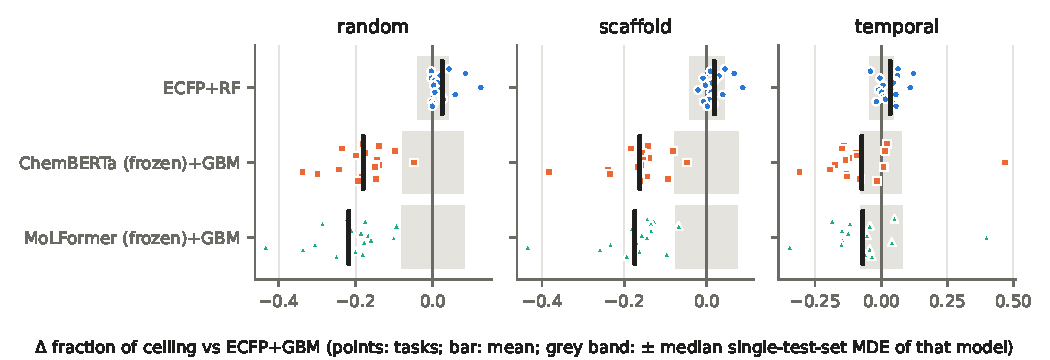
\includegraphics[width=\linewidth]{figures/paired_diff.pdf}
\caption{Per-task difference in fraction of ceiling relative to ECFP+GBM (points: tasks; bar: mean over tasks; grey band: $\pm$ median single-test-set MDE of each model).}\label{fig:paired}\end{figure}

\begin{figure}[ht]\centering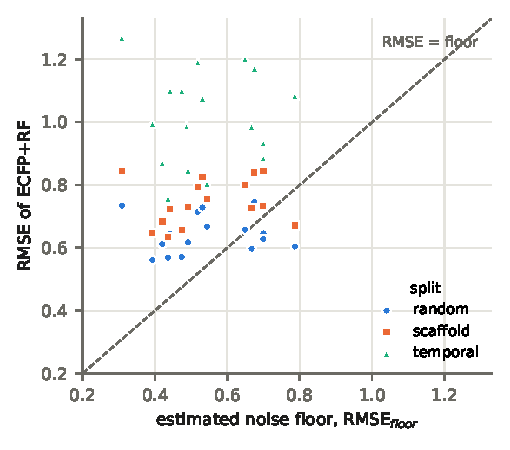
\includegraphics[width=0.5\linewidth]{figures/floor_vs_rmse.pdf}
\caption{Estimated noise floor versus test RMSE of ECFP+RF per task and split. Points below the dashed line have RMSE below the estimated floor ($f>1$).}\label{fig:floor}\end{figure}

\begin{table}[ht]\centering\small\setlength{\tabcolsep}{4pt}\caption{Mean fraction of ceiling $f$ over tasks ($n$ = number of tasks), decontaminated data. Models with $n<17$ were run on a subset of tasks and are not comparable with the rest (see Table~\ref{tab:subset}).}\label{tab:frac}
\begin{tabular}{lcccc}\toprule Model & $n$ & Random & Scaffold & Temporal\\\midrule
ECFP+GBM & 17 & 0.87 & 0.71 & 0.32\\
ECFP+RF & 17 & 0.90 & 0.73 & 0.36\\
ECFP+MLP & 17 & 0.47 & 0.18 & -0.51\\
ChemBERTa-77M (frozen)+GBM & 17 & 0.69 & 0.55 & 0.25\\
MoLFormer-XL-10\% (frozen)+GBM & 17 & 0.66 & 0.54 & 0.25\\
D-MPNN & 5 & 0.63 & 0.54 & 0.27\\
ChemBERTa-77M (fine-tuned) & 5 & 0.60 & 0.49 & 0.31\\
\bottomrule\end{tabular}\end{table}

\begin{table}[ht]\centering\small\setlength{\tabcolsep}{4pt}\caption{Paired difference in $f$ versus ECFP+GBM over 17 tasks (positive = better than ECFP+GBM); Wilcoxon signed-rank test, Holm-adjusted $p$.}\label{tab:paired}
\begin{tabular}{llccc}\toprule Model & Split & mean diff. & better on & $p_{\text{Holm}}$\\\midrule
ECFP+RF & random & +0.024 & 13/17 & 0.013\\
ECFP+RF & scaffold & +0.019 & 13/17 & 0.033\\
ECFP+RF & temporal & +0.034 & 13/17 & 0.032\\
ECFP+MLP & random & -0.400 & 0/17 & $<$0.001\\
ECFP+MLP & scaffold & -0.535 & 0/17 & $<$0.001\\
ECFP+MLP & temporal & -0.836 & 0/17 & $<$0.001\\
ChemBERTa-77M (frozen)+GBM & random & -0.181 & 0/17 & $<$0.001\\
ChemBERTa-77M (frozen)+GBM & scaffold & -0.163 & 0/17 & $<$0.001\\
ChemBERTa-77M (frozen)+GBM & temporal & -0.074 & 4/17 & 0.033\\
MoLFormer-XL-10\% (frozen)+GBM & random & -0.218 & 0/17 & $<$0.001\\
MoLFormer-XL-10\% (frozen)+GBM & scaffold & -0.175 & 0/17 & $<$0.001\\
MoLFormer-XL-10\% (frozen)+GBM & temporal & -0.070 & 3/17 & 0.033\\
\bottomrule\end{tabular}\end{table}

\begin{table}[ht]\centering\small\setlength{\tabcolsep}{4pt}\caption{Mean $f$ on the 5 tasks where D-MPNN (3 seeds) and fine-tuned ChemBERTa (3--5 seeds) were run (CHEMBL204\_Ki, CHEMBL206\_IC50, CHEMBL214\_Ki, CHEMBL237\_IC50, CHEMBL237\_Ki); all models on the same tasks.}\label{tab:subset}
\begin{tabular}{lccc}\toprule Model & Random & Scaffold & Temporal\\\midrule
ECFP+GBM & 0.73 & 0.61 & 0.25\\
ECFP+RF & 0.76 & 0.63 & 0.28\\
ECFP+MLP & 0.36 & 0.07 & -0.41\\
ChemBERTa-77M (frozen)+GBM & 0.61 & 0.49 & 0.27\\
MoLFormer-XL-10\% (frozen)+GBM & 0.58 & 0.47 & 0.23\\
D-MPNN & 0.63 & 0.54 & 0.27\\
ChemBERTa-77M (fine-tuned) & 0.60 & 0.49 & 0.31\\
\bottomrule\end{tabular}\end{table}

\begin{table}[ht]\centering\small\setlength{\tabcolsep}{4pt}\caption{Effect of decontamination: mean $f$ on decontaminated and uncleaned data and mean change in test RMSE (uncleaned $-$ decontaminated) over 17 tasks.}\label{tab:leak}
\begin{tabular}{llccc}\toprule Model & Split & $f$ clean & $f$ uncleaned & $\Delta$RMSE\\\midrule
ECFP+GBM & random & 0.87 & 0.90 & +0.000\\
ECFP+GBM & scaffold & 0.71 & 0.74 & -0.005\\
ECFP+GBM & temporal & 0.32 & 0.35 & -0.003\\
ECFP+RF & random & 0.90 & 0.92 & +0.002\\
ECFP+RF & scaffold & 0.73 & 0.75 & +0.000\\
ECFP+RF & temporal & 0.36 & 0.38 & -0.005\\
ECFP+MLP & random & 0.47 & 0.47 & +0.009\\
ECFP+MLP & scaffold & 0.18 & 0.15 & +0.022\\
ECFP+MLP & temporal & -0.51 & -0.47 & -0.025\\
ChemBERTa-77M (frozen)+GBM & random & 0.69 & 0.71 & +0.006\\
ChemBERTa-77M (frozen)+GBM & scaffold & 0.55 & 0.56 & +0.005\\
ChemBERTa-77M (frozen)+GBM & temporal & 0.25 & 0.26 & +0.004\\
MoLFormer-XL-10\% (frozen)+GBM & random & 0.66 & 0.67 & +0.005\\
MoLFormer-XL-10\% (frozen)+GBM & scaffold & 0.54 & 0.55 & -0.000\\
MoLFormer-XL-10\% (frozen)+GBM & temporal & 0.25 & 0.27 & -0.002\\
\bottomrule\end{tabular}\end{table}

\section{Recommendations}\label{sec:recs}
\paragraph{Minimum detectable effect.}
For a paired comparison of two models on one test set of $n$ molecules, with per-molecule differences of squared errors $d_i=e_{A,i}^2-e_{B,i}^2$, the smallest MSE difference detectable at level $\alpha$ with power $1-\beta$ is approximately $(z_{1-\alpha/2}+z_{1-\beta})\,\mathrm{sd}(d)/\sqrt{n}$; dividing by $2\,\mathrm{RMSE}_B$ converts it to RMSE units (delta method), and dividing by $\mathrm{RMSE}_{\text{mean}}-\mathrm{RMSE}_{\text{floor}}$ to units of $f$. On our test sets (200--1{,}900 molecules) the median MDE ($\alpha=0.05$, power 0.8) is about 0.04 in $f$ for ECFP+RF versus ECFP+GBM, whose errors are strongly correlated, and about 0.08 for frozen embeddings versus ECFP+GBM (\texttt{results/full\_clean/mde.csv}). Differences smaller than this on a single dataset should not be reported as improvements; detecting them requires pooling over tasks with a paired test, as we do here. The approximation assumes independent test molecules; molecules from the same document or series have correlated errors, so these MDEs are optimistic. It has not been validated by simulation.

\paragraph{Reporting protocol.}
For each task, report: the estimated between-document standard deviation with confidence intervals from a bootstrap over document pairs, the number of replicated molecules and of distinct document pairs, the trimming rule, and how duplicated values and stereoisomers were handled; $f$ alongside RMSE and $R^2$; the ChEMBL release and retrieval date; split type and seeds; paired differences against a tuned ECFP baseline with a test over tasks; and the decontamination performed (exact, connectivity and near-analogue matches against public benchmarks; status of pretraining-corpus overlap).

\paragraph{Checklist.}
\begin{itemize}[nosep]
\item Are replicates from independent documents, and how many molecules have them?
\item Is the floor computed for the test molecules, with a confidence interval over document pairs and sensitivity to trimming and duplicated values?
\item Is the ECFP baseline tuned with the same budget as the proposed model?
\item Are random, scaffold and temporal splits and at least five seeds reported?
\item Is every $f>1$ investigated (leakage, within-document effects, floor estimate) rather than reported as success?
\item Is overlap of the test set with pretraining data checked, or stated as unknown?
\item Is the claimed improvement larger than the minimum detectable effect, or tested across tasks?
\end{itemize}

\section{Limitations}\label{sec:limits}
\begin{itemize}
\item \textbf{The floor is cross-document variability, not instrument error.} It includes systematic differences between assays and laboratories and curation errors. Relative to a single well-controlled assay it overstates the irreducible error; relative to a model that can learn document-specific offsets (random splits) it may also be too pessimistic, as the cases with $f>1$ show. We have not yet evaluated document-grouped splits, which would separate these effects.
\item \textbf{Dependence and representativeness of replicates.} The floor is estimated from the 1.8--11.1\% of molecules that were measured in several documents. These are more potent on average than other molecules in several tasks, are concentrated in few document pairs for some tasks (one pair contributes 79\% of molecule pairs for CHEMBL237 $\mathrm{IC}_{50}$), and include identical values that are probably re-publications. We assume one noise variance per task. Shared authors, re-published values and assay conditions (substrate or ATP concentration, species, mutants) were not checked.
\item \textbf{Sensitivity to curation choices.} The estimated noise depends on the trimming threshold, on how duplicated values and stereoisomers are treated and on assay selection (Table~\ref{tab:robust}); for some tasks these choices change $\hat s$ by 0.1 or more. The assay confidence threshold of 8 admits homologous proteins.
\item \textbf{Leakage.} Decontamination covers MoleculeNet and TDC but not Polaris datasets or the pretraining corpora of the foundation models, which are large subsets of PubChem and ZINC and may contain test molecules. Such overlap would be expected to favour the pretrained models, which nevertheless perform worse. Removing MoleculeNet and TDC molecules changed test errors very little (Section~\ref{sec:results}).
\item \textbf{Model coverage.} We test two small chemical language models, frozen, on all tasks and only a D-MPNN and one fine-tuned model on five tasks with three seeds; larger or more recent foundation models, other heads and longer hyperparameter searches may behave differently. The hyperparameter budget (three configurations) is small for all models.
\item \textbf{Splits.} The temporal split leaks some information (ties at the cut-off year; training labels include later documents), and the inner validation split used for hyperparameters is random for all outer splits.
\item \textbf{Scope.} Potency endpoints ($K_i$, $\mathrm{IC}_{50}$) from ChEMBL only; we make no claim about ADMET or physicochemical endpoints. $K_i$ and $\mathrm{IC}_{50}$ tasks also differ in target class (mostly GPCRs versus mostly kinases), so differences between them are not attributable to the measurement type alone. Test labels are noisy; we do not correct test metrics for attenuation.
\item \textbf{Literature.} Our account of related work is based on the published abstracts and metadata of several cited papers; we did not reproduce their analyses.
\end{itemize}

\section{Datasheet and metadata}
\paragraph{Track requirements.}
From the NeurIPS 2025 D\&B call page (fetched; the 2026 D\&B call page returned 404, so \emph{2026 requirements are not verified}): authors should provide machine-readable metadata in the Croissant format with the OpenReview submission (auto-generated on Kaggle, OpenML, Hugging Face, Dataverse; otherwise self-generated and validated); datasets hosted on one of these platforms or a bespoke site and accessible to reviewers without personal request; executable code on GitHub or similar; public availability by camera-ready. Page limit and checklist for D\&B 2026: not verified (the main-track 2026 page lists a template archive but not the limit). Whether a datasheet is mandatory: not verified; we include one regardless \todo{check 2026 call and checklist.tex}.
\paragraph{Style file.}
The archive \texttt{Formatting\_Instructions\_For\_NeurIPS\_2026.zip} (media.neurips.cc) was downloaded and contains \texttt{neurips\_2026.sty}, \texttt{neurips\_2026.tex}, \texttt{checklist.tex}. Its D\&B-specific options were not checked.
\paragraph{License.}
The ChEMBL FTP README states data are licensed under Creative Commons Attribution-ShareAlike 3.0 Unported (CC BY-SA 3.0). Derived data release thus should carry share-alike terms and attribution; legal review \todo{confirm}. Code licence: \tbd{}.
\paragraph{Datasheet items (to fill).}
Motivation; composition (molecules, endpoints, documents); collection process (ChEMBL release \tbd, date \tbd, API); preprocessing; uses and misuses (not a substitute for experimental validation; ceilings are cross-source, not instrument, limits); distribution (host \tbd, DOI \tbd, Croissant file \tbd); maintenance and contact \tbd; personal data: none expected (compound data) --- to confirm.

% Bibliography: paper/references.bib (W8). Until it exists, \cite{TODO-...} render as [?].
\IfFileExists{references.bib}{\bibliographystyle{plain}\bibliography{references}}{}
\end{document}
